% Compile with pdflatex. The editable figure is included below.
\documentclass[11pt,letterpaper]{article}
\usepackage[T1]{fontenc}
\usepackage[utf8]{inputenc}
\usepackage{lmodern,microtype,tikz,hyperref,fancyhdr}
\usepackage[margin=0.88in,headheight=14pt,headsep=12pt]{geometry}
\usepackage[compact]{titlesec}
\definecolor{ink}{HTML}{1C4448}
\definecolor{steel}{HTML}{CBDCDA}
\definecolor{accent}{HTML}{883948}
\hypersetup{colorlinks=true,urlcolor=ink,linkcolor=ink}
\titleformat{\section}{\sffamily\Large\bfseries\color{ink}}{}{0pt}{}
\titleformat{\subsection}{\sffamily\normalsize\bfseries\color{ink}}{}{0pt}{}
\setlength{\parindent}{0pt}
\setlength{\parskip}{0.54em}
\setlength{\emergencystretch}{1.5em}
\pagestyle{fancy}\fancyhf{}\lhead{\small\sffamily NSF AMDO}\rhead{\small\sffamily Provisional project description}\rfoot{\small\sffamily Collaborative working draft\quad\thepage}
\begin{document}

\section*{Stock Allocation for Distortion Control in Thin-Plate Machining}

A thin aluminum plate can meet its thickness specification under clamps and fail its flatness specification after release. While both faces still carry excess stock, the machinist can remove more from either face and leave the finished thickness unchanged. The choice determines which layers of metal remain. To see how the unfinished plate bends, the machinist can remove the clamps and measure its free shape. Doing so costs a setup and can change how the plate sits for the next cut.

\subsection*{Which plate warrants another setup?}

A released shape records the bending effect of stresses through the remaining thickness. Two plates can have the same bow while carrying stress at different depths. Cutting a layer from the same face can then drive one plate toward its drawing and the other away from it. We propose to learn when the known stock origin and cutting history resolve this ambiguity and when observing released shape changes the better allocation. The practical test is whether the resulting choice improves conformance enough to justify the interruption.

\begin{center}

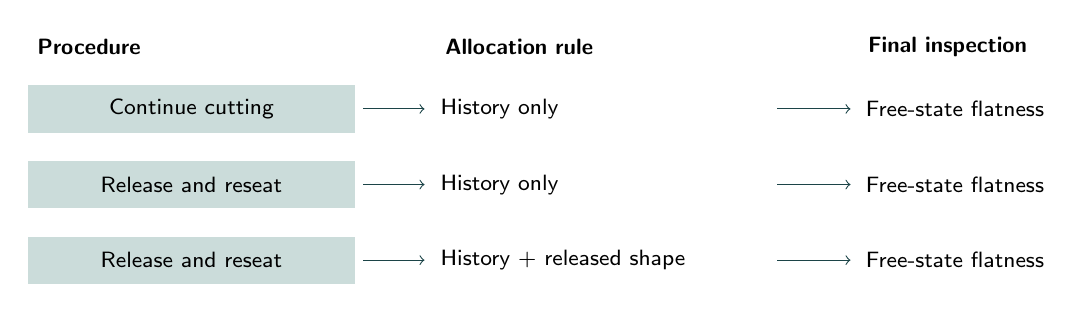
\begin{tikzpicture}[x=1cm,y=1cm,font=\sffamily\footnotesize,every node/.style={align=center}]
\node[anchor=west,font=\sffamily\bfseries\footnotesize] at (0,2.84){Procedure};
\node[anchor=west,font=\sffamily\bfseries\footnotesize] at (5.18,2.84){Allocation rule};
\node[anchor=west,font=\sffamily\bfseries\footnotesize] at (10.55,2.84){Final inspection};
\foreach \y/\procedure/\rule in {2.05/Continue cutting/History only,1.09/Release and reseat/History only,0.13/Release and reseat/History + released shape}{
  \fill[steel] (0,\y-.30) rectangle (4.16,\y+.30);
  \node at (2.08,\y){\procedure};
  \draw[->,ink] (4.26,\y)--(5.04,\y);
  \node[anchor=west] at (5.12,\y){\rule};
  \draw[->,ink] (9.52,\y)--(10.45,\y);
  \node[anchor=west] at (10.52,\y){Free-state flatness};
}
\end{tikzpicture}

\end{center}

{\small\textbf{Figure 1.} Both reseated arms receive the same scan. Revealing its result changes only the information available when selecting a face split. All three arms receive blinded final inspection.}

Hao et al. used online deformation readings to update allowances on alternating faces [1]. Li et al. developed a fixture that responds to workpiece deformation during machining [2]. An NSF GOALI award also coupled residual-stress estimation and tool-path design [4]. Our design will prioritize new cuts where plausible stress profiles favor opposite faces and the predicted difference matters to the drawing. We will compare this allocation of experiments with balanced sampling at the same machining budget.

\newpage

\section*{Aim 1 · Test for reversals in the better finishing cut}

\textbf{Year 1.} Satish Bukkapatnam's group will qualify one functioning CNC mill, one two-sided fixture and an independent gauge for final free-state flatness. The shop must confirm on its drawing that the final mid-plane may shift and both faces retain sufficient cleanup stock under either split. The group has demonstrated motion sensing on a Langmuir MR-1 [7], and Texas A\&M lists shared CNC equipment [5]. Qualification requires a staffed cut under load at the proposed dimensions, traceable stock, and repeated release, support and reseating trials. Set the support span and release sequence to the shop's best feasible practice, since unclamping itself can alter the measured shape [9]. Time that setup, quantify gauge scatter on repositioned parts and check thermal effects. If fixture correction alone meets the drawing, end the production trial.

\subsection*{Cross the face split with recorded stock origin}

We will cut sibling blanks from neighboring mapped positions in independent parent plates. Mark the original face and rolling direction, record the through-thickness origin, and apply a common roughing cut within each stock level. Before finishing, measure the full released profile on repeatable supports. At each tested level retain two preregistered allocations with the same total removal and final thickness. Randomize individual blanks to those splits within parent, origin and stock-level blocks. Each blank supplies a final flatness and a signed curvature along the marked axis under one allocation. A treatment contrast requires several independently cut blanks in each arm.

We will test two complementary predictions. Among blanks with profiles alike within an equivalence band set from gauge repeatability, does stock origin and prior removal history predict that opposite splits work best? Within a common recorded history, do distinguishable profiles predict a reversal? The first test identifies what a shape-only rule misses. The second identifies a reason to buy the reading. Before cutting, the shop will specify a useful reduction in final free-state flatness error in millimeters. A reversal requires greater removal from the marked face to reduce this unsigned error by that margin in one group and greater removal from the opposite face to do so in another. Signed curvature records the direction of bending for the mechanics test.

\subsection*{First decision on experimental scale}

Bukkapatnam will deliver the cut records, timed reseats and uncertainty of the independent gauge to Rui Tuo and Xianyang Zhang. Zhang will estimate sibling and parent variation to determine how many parent plates can resolve a useful reversal. If the drawing prevents a second allocation, the measurement obscures that margin, or the required independent stock exceeds the available campaign, the full trial loses its experimental basis.

\newpage

\section*{Aim 2 · Identify which observations change the cut}

\textbf{Year 2.} Tuo will predict the difference in final flatness between the same two allocations at a specified stock level. One model propagates an inherited through-thickness stress profile as the two faces are removed. The other also allows the preceding cuts to alter stress in a shallow surface layer. Two candidate profiles can give indistinguishable relaxed shapes if their bending moments agree. Removing a slice changes both its share of that moment and the stiffness of what remains. This gives the models a physical opportunity to predict different responses on the next cut.

Tuo will rank feasible experiments by the expected reduction in drawing loss on future jobs per staffed minute. Competing stress profiles receive weights calibrated on development stock. Their disagreement matters most where plausible profiles favor different face splits and the wrong split has a material flatness penalty. Bukkapatnam will create a bank of randomized sibling cuts covering the prespecified histories, stock levels and splits. From the same initial cuts, each design can reveal only the measured outcomes it requests, up to the same time budget. The balanced design cycles across histories and splits. Both use the same model, fitting procedure and feasible actions. Zhang will reserve independent parents for comparing the resulting rules [6].

\subsection*{Check the mechanical explanation independently}

Randomized cuts can establish which allocation performs better. Attribution to inherited or machining-induced stress requires an additional observation. Subject to qualification, sacrificial matched blanks will supply a separate bulk-stress estimate from incremental layer removal and surface-stress measurements after roughing by X-ray diffraction. On parent stock reserved for this test, we will compare measured signs, depths and uncertainty with predictions recorded before testing [3,8]. Both methods sample siblings, so a model that predicts the better allocation but misses the stress observations supports a decision rule only. If the reference measurements are unavailable, the stress-source attribution remains open.

\subsection*{Freeze what the operator can know}

On randomized development cuts, benchmark a fixed split, the shop’s ordinary rule, a deformation-series rule adapted from Hao et al. [1], and a reduced-layer-removal predictor [3]. Give the Hao adaptation its sequence of in-process readings and charge the time to obtain them. Record any readings the pilot setup cannot reproduce. Year 3 compares against the best rule implementable without an extra release. A claim of superiority to the instrumented method would require a direct comparison on new stock. Before evaluating either design, specify the job mix and use a common conversion for setup time and drawing loss agreed with the shop. Freeze both designs' rules for stopping and choosing a cut. Each stop decision can use only information already available under clamps.

\newpage

\section*{Aim 3 · Measure the return on one interruption}

\textbf{Year 3.} Reserve complete parent plates before model fitting. On each validation blank, log the frozen stop decision before releasing any clamp. Where the rule calls for a stop, randomize within parent and stock level to continuous machining, release/scan/reseat with the reading withheld, or the same procedure with the reading visible. The first two use the frozen history-only split. The third may use the new reading. Where the rule calls for continuing, follow that route and retain those blanks in the overall estimate. A blinded inspector will grade every released plate on the same supports after thermal equilibration.

Zhang will report drawing yield, flatness error, hands-on operator time and occupied mill time. Visible versus withheld readings estimate the benefit of the data. Withheld versus continuous cutting estimates the effects of handling and delay. Visible versus continuous estimates the operational gain in the stop region. Both policies use continuous history-only machining on other jobs. Zhang will weight the stop-region contrasts within stock and history strata by their frequencies in the predefined shop workload. This estimates the complete policy's gain over continuous history-only machining. Uncertainty will reflect whole parents and within-parent randomization. In a separate reserved subset, randomize blanks before any scan to the complete rule learned from targeted or balanced cuts. Sample from the same predefined workload. Their difference in drawing loss and time measures what the experimental design bought. Size both comparisons from the pilot.

\subsection*{What a shop can use}

The shop will receive a table for the tested drawing and stock origins showing when to measure and which face to cut. It will flag conditions where either split meets the shop’s margin and those where uncertainty still admits a consequential loss. We will report additional machine minutes per reject avoided when yield improves, and convert that estimate to a break-even reject cost if the shop supplies an hourly rate. Machining students will choose cuts for unseen plates before and after instruction. Blinded drawing grades and setup minutes will measure improvement on matched exercises. The three-year scientific case ends if a fixed or history-only split performs equivalently even in predicted reversal cases. A resolved reversal with no net economic gain would support the physical finding while favoring continued machining. Intervals spanning meaningful benefit and harm leave the decision unresolved.

\subsection*{Selected sources}

\begin{enumerate}
\small\setlength{\itemsep}{0pt}
\item \href{https://doi.org/10.1016/j.cja.2020.03.038}{Hao et al. (2020). An allowance allocation method based on dynamic approximation via online inspection data for deformation control of structural parts.}
\item \href{https://doi.org/10.1016/j.cirp.2015.04.025}{Li et al. (2015). Responsive fixture design using dynamic product inspection and monitoring technologies for the precision machining of large-scale aerospace parts.}
\item \href{https://doi.org/10.3390/jmmp8010009}{Aurrekoetxea et al. Machining distortion prediction from reduced layer removal.}
\item \href{https://www.nsf.gov/awardsearch/showAward?AWD_ID=1762722}{NSF. GOALI machining distortion project, award 1762722.}
\item \href{https://texasmakes.tamu.edu/facilities/}{Texas A\&M. Institute for Manufacturing Systems facilities.}
\item \href{https://arxiv.org/abs/2604.17144}{Li, Zhang and Tuo. Physical model validation against observations. Preprint, 2026.}
\item \href{https://ssrn.com/abstract=7243783}{Hanchate et al. Machine-tool digital twin architecture and validation. Preprint, 2026.}
\item \href{https://doi.org/10.1007/s11340-021-00734-5}{Chighizola et al. Comparing near-surface stress measurements in milled aluminum.}
\item \href{https://link.springer.com/article/10.1007/s00170-026-17756-9}{Casuso et al. Multistage laser measurement of thin aluminum plates.}
\end{enumerate}

\end{document}
